% !TEX root = ../main.tex
% Chapter Background information and theory

\chapter{State-of-the-art of conversational agents systems} % Main chapter title
% \chapter{Background information and theory} % Main chapter title

\label{Chapter2} % Change X to a consecutive number; for referencing this chapter elsewhere, use \ref{ChapterX}

A conversational agent (chatbot) is intended to respond to a Human by taking advantage of all its knowledge, its capacity to detect sentiments or remember the context, or its ability to search information on the web. Chatbots tend to use text as input and output format but it is also possible to use speech recognition and speech generation to allow users to speak.

\section{Different approaches to build a conversation agent}
Chatbots are created using two different approaches, namely the \textbf{Rule-based} approach and the \textbf{Generative} approach. The Rule-based approach, as its name indicates, uses rules to understand user input and pick from a list of possible answer to reply to him. Rule-based chatbots exist since 1966 with the developement of ELIZA chatbot in \cite{Weizenbaum:1966:ECP:365153.365168}. ELIZA's goal was to measure the psychological effects on Humans when they talk to a machine. Some of the test subjects found it really hard to believe that they were talking to a computer. ELIZA follows a script and analyzes user input to find keywords and to choose the proper answer. The workload for the developper is quite intensive and it only takes one wrong answer that the developer might not have thought of and the user understands he is not talking to a Human.

The Generative approach is a machine learning model that takes advantage of the recent research and technology improvements enabling deep neural networks model to be trained on large datasets. The main difference with the rule-based approach is that the chatbot learns and establishes its own rules based on the training dataset. Thus, generative models are less entitled to misunderstand the user but since they learn themselves the output sentences, they might generate sentences with punctuation errors, grammatical errors, or even generate incomprehensible sentence. Aside the generation problems, training deep neural networks is not an easy task and require high performance hardware.

These two approaches are used in two different cases, closed-domain and open-domain conversations. The closed-domain conversation means that the chatbot can answers to a particular type of questions. For example, a company develops a chatbot to let users manage their booking details will only be able to answer requests about bookings and nothing else. At contrary, an open-domain chatbot is able to discuss about anything. For example, Siri the personnal assistant developed by Apple or Alexa the personnal assistant developed by Amazon are able to understand very different requests and they are not blocking the user. Figure \ref{fig:types_chatbot} shows the different types of chatbots and hightlights the fact that the rule-based approach is only meant for closed-domain conversations. An open domain chatbot based on prepared scenarios and answered and following rules is impossible due to the amount of work needed to construct such a system.

\begin{figure}
    \centering
    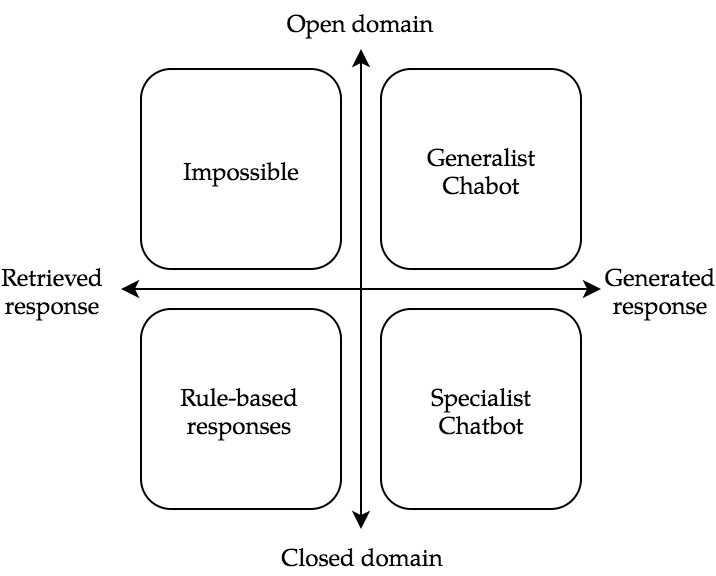
\includegraphics[width=.66\textwidth]{types_chatbot}
    \caption{Different types of chatbot.}
    \label{fig:types_chatbot}
\end{figure}

\section{Rules-based models}
Technology from 1970's, AIML, etc.

\section{Generative approach}
Generative conversation models are based on a learning process and need a large set of training data (e.g. \cite{1506.05869} used 62M sentences). Generative models are created using deep neural networks like Recurent Neural Network (RNN) \citep{1503.02364,1506.05869}. Since

\subsection{Neural Network}
Neural Network (NN) is a statistical machine learning model that uses weights and activation functions to mimic the biological neuronal system. The

\subsection{Long Short-Term Memory}
Recurrent Neural Network (RNN) is a deep neural network created to deal with time-series.

\subsection{Neural Machine Translation}
Sequence-to-sequence (Seq2Seq) \citep{1409.3215} was first introduced by Google to be an end-to-end approach that makes only minimal assumptions on the sequence structure. In the use case of chatbots, it means that the input and output sequences, or conversations, can have basically any length and the NN is still able to learn. Seq2Seq approach decompose the architecture in two main parts, namely the encoder and the decoder. The encoder takes as input a sequence of text and forms an abstract representation of it. The decoder uses this abstract representation produced by the encoder to output the adequate output sentence. The abstract representation is meant at capturing relevant information from the input sentence. Figure~\ref{fig:nmt} presents the workflow of a NMT model. The example shown is a translation problem, but NMT model architecture is used also for conversational agents or text summarization \citep{tensorflow.nmt}.

\begin{figure}
    \centering
    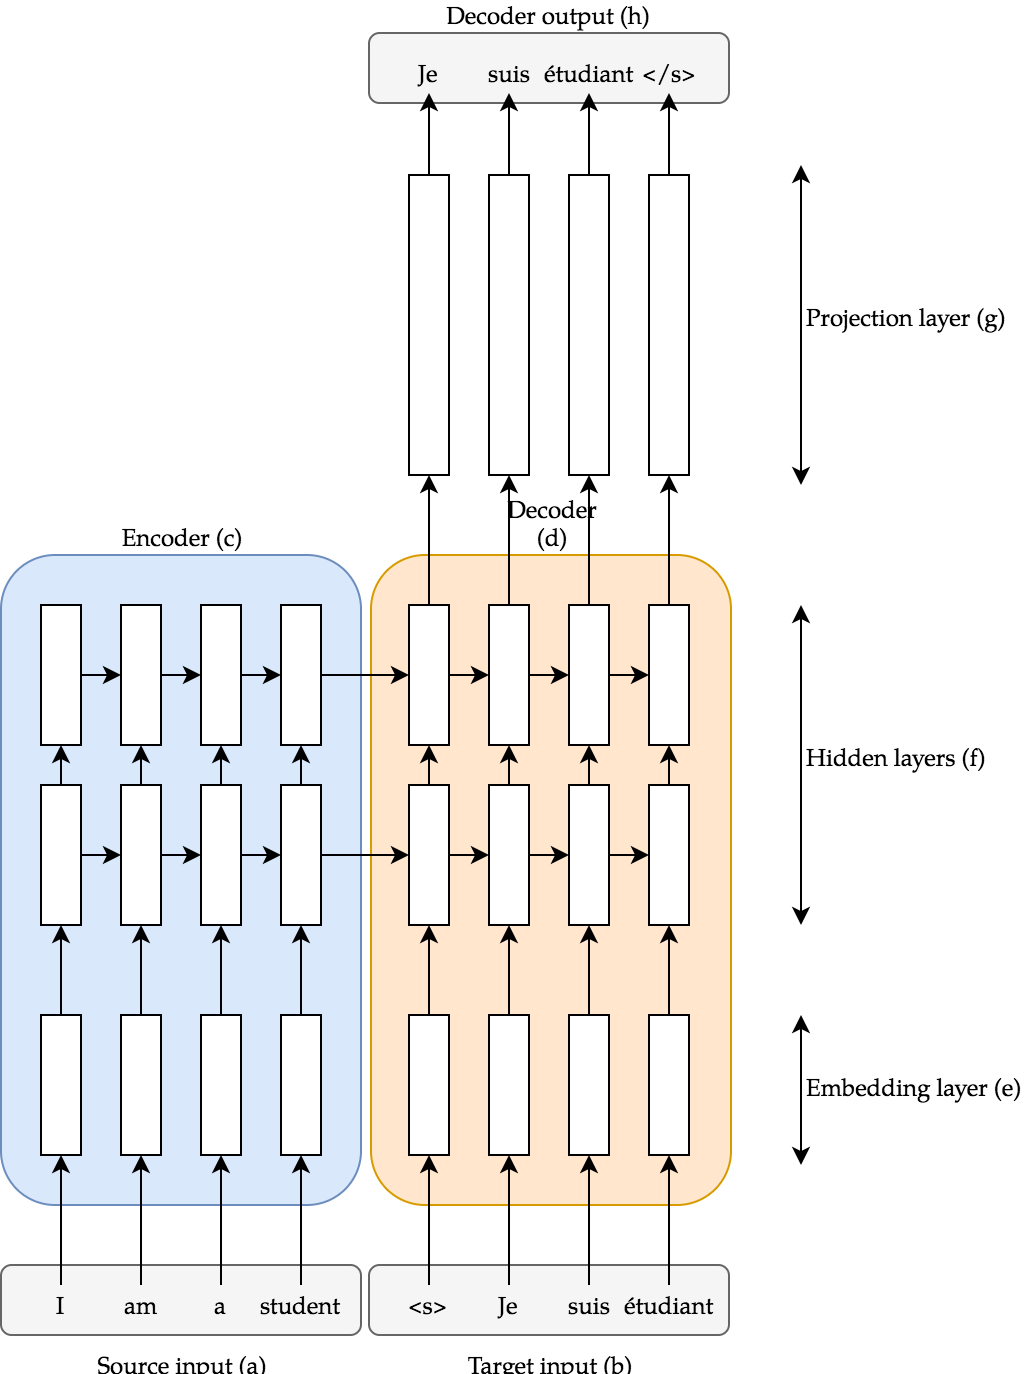
\includegraphics[width=.8\textwidth]{nmt_training_scheme}
    \caption{Neural Machine Translation model \citep{tensorflow.nmt}. \textbf{(a)} \textit{Source input} refers to the input sequence tokenized to let the encoder read it token by token. \textbf{(b)} \textit{Target input} refers to the decoder input that let the decoder have the correct $t-1$ token and decode properly. \textbf{(c)} \textit{Encoder} refers to stacked RNN model used to build an abstract representation of the input sequence. \textbf{(d)} \textit{Decoder} refers to stacked LSTM that produce the output sequence based on the abstract representation built by the encoder and on the ``previous'' target word. \textbf{(e)} \textit{Embedding layer} refers to the feedforward neural network language model that creates words' vector representation. \textbf{(f)} \textit{Hidden layers} refers to the number of stacked RNN layers. \textbf{(g)} \textit{Projection layer} refers to the one-hot vector of the predicted word, used to calculate the loss. \textbf{(h)} \textit{Decoder output} refers to the output sequence tokenized.}
    \label{fig:nmt}
\end{figure}

Both the encoder and the decoder are RNN: LSTMs \citep{1409.3215,1508.04025} or GRUs \citep{1706.05125,1503.02364}. As LSTMs take real vectors as inputs, the text sequence has to be represented as continuous vectors, known as word embeddings. A technic called word2vec, developped \citep{1301.3781}, proposed two log-linear models based on Feedforward Neural Net language Model (NNLM) to represent efficiently words in vector space. The first model architecture of word2vec is called the Continuous Bag-of-Words (CBOW) model and follow the feedforward NNLM architecture with one hidden layer. The idea behind is that we train a model to predict a word from a sentence using the two words occuring before and two occuring after it in the sentence (e.g. in ``\textit{This corpus contains millions entities}'', the input's model are \textit{This, corpus, millions entities} and the target is \textit{contains}). Figure~\ref{fig:cbow} shows the CBOW architecture. The skip-gram architecture, represented in Figure~\ref{fig:skipgram}, takes as input the current word to predict the context. Empirical results \citep{tf.word2vec} show that the Skip-gram model is more useful for large datasets as for CBOW, it fits better on small datasets.

\begin{figure}
    \centering
    \begin{subfigure}{.45\textwidth}
        \centering
        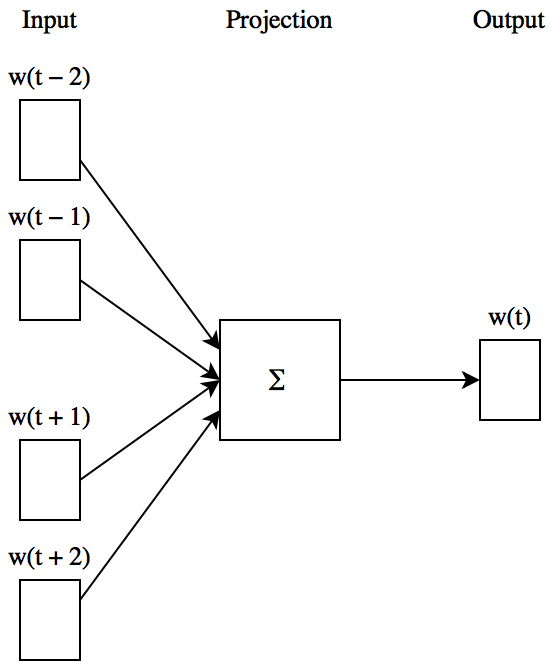
\includegraphics[width=.8\textwidth]{word2vec_cbow}
        \caption{CBOW architecture from word2vec models. Context is used to predict the current word.}
        \label{fig:cbow}
    \end{subfigure}
    ~
    \begin{subfigure}{.45\textwidth}
        \centering
        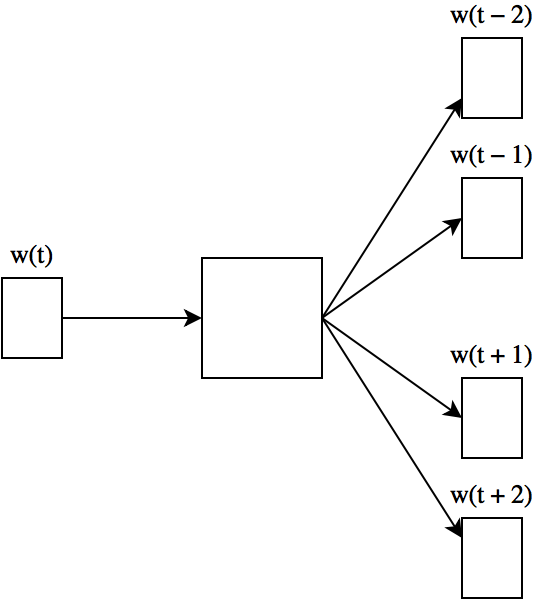
\includegraphics[width=.8\textwidth]{word2vec_skipgram}
        \caption{Skip-gram architecture from word2vec models. Current word is used to predict the context.}
        \label{fig:skipgram}
    \end{subfigure}
    \caption{Word2vec architectures.}
    \label{fig:word2vec}
\end{figure}

One important parameter of the word2vec model is the dimension of the vector space where the model represents the words. The default and used sizes of the vector space vary between 100 (ref Keras) and 300 (ref word2vec google).

\section{Development tools}
dialogflow.com, wit.ai

\section{Generative models}
The generative models approach of constructing a chatbot takes advantage of recent research work in DNN and NLP. Before training a neural network, the text has to be represented in term of a vector, and different approaches exist for it.
The bag-of-word (BOW) model idea is to count the different tokens present in the dataset and create a vector of all these tokens.

Word embeddings is a trainable feature that allows to put together words having the same meaning or having the same role in a text. The words are represented by vectors between 100 and 300 components \textbf{ref needed for the numbers}. For example, \textit{queen} - \textit{king} + \textit{man} = \textit{woman}.


\section{Encoding text}
Machine learning models are mathematical models, therefore methods have been developped to encode text as vectors. Bag-of-words (BOW) is indexing all the unique words of the corpus and for each input sequence, counts the number of times any unique words appears or not. This process creates a vector very sparse that have a majority of zeros. the counting has different forms : term frequency (tf) and term frequency over inverse document frequency (tf-idf). Tf is straightforward because it counts simply the number of times each word appear. Tf-idf is taking into account the rarity of the words appearing. For instance, if a word appears only in two different sequence of the corpus and one time in the current sequence, the tf-idf score will be higher than another word that would appear in almost all the documents of the corpus.

Word embeddings is a trainable encoding process. The main idea is to represent into a fixed size space (e.g. 300 \textbf{REF}, 100 \textbf{REF}) all the words of the corpus. The results show that different words linked together are clusterized into different group of meaning and their vector representation carry this information allowing in some cases basic algebraic operation (e.g. \textit{queen} - \textit{king} + \textit{man} = \textit{woman}). Word embeddings add the notion of similarity between words instead of treating words as atomic units \citep{1301.3781}.

\section{Tokenize input text}
Words chunks, character, syllabls

\section{Dropout}
1409.2329 shows that dropout (UofT, srivastava, 2013) does not work well with RNNs. Moreover, people tend to use small RNNs models because large one tend to overfit. 1409.2329 answers these problems by applying dropout to a certain subset of the RNNs' connections (blabla how they used dropout differently on RNN and LSTM)

\section{RNN with varying input length}
Different technics : padding, bucketing, dynamicRNN (TensorFlow)

What is a conversational agent (Chatbot)
The two approaches of a chatbot "construction" (markup language and generative models)

Explain the following:
NLP (word2vec) / Feature engineering / word embedding
Neural Nets / RNN (with the vanishing gradient problem, problematic in long conversations, ref needed) / LSTM / Attention Mechanism
seq2seq model (Best practices on the architecture of a seq2seq model)/ Machine Translation models / NeuralMT by Google nov '16 with an end-to-end training
Greedy search / Beam search
evaluation model (BLEU score) / present paper on how NOT evaluate / perplexity
empathic conversational agent (apr 17)

State-of-the-art
state-of-the-art on conversations generation

\section{RNN}
Bengio et al. (1994) detail vanishing and exploding gradient problems of RNN
1211.5063 answers exploding gradient problem with gradient clipping


Issue with the non-presence of an <EOS> (end-of-sequence) (it can be a special character like a \textbackslash t or \textbackslash n) => the decoder generates character/words as the longest input sequence it received

\section{Unknown words in a n-grams count based language model}
1703.01619 present three common ways to deal with unknown words, or in other terms, words not present in the training set vocabulary. 1) Assume closed vocabulary. It means that we simply aknowledge that our model will not be able to output words out of the vocabulary and therefore will not be able to recognize them. 2) Interpolate with an unknown words distribution. \textbf{dunno yet what it means} 3) Add an unk token \citep{1703.01619}

\section{Amazon Alexa}
Present the paper and how does a model for Alexa works? => Dialogue manager with submodels that takes care of ONE job and the dialogue manager calculates the probability for the submodels to really answer the question. Submodels also provide a confidence score to help the dialogue manager?
